\documentclass[12pt,a4paper]{article}
\usepackage[utf8]{inputenc}
\usepackage[english]{babel}
\usepackage{enumerate}
\usepackage{amsmath}
\usepackage{amsfonts}
\usepackage{amssymb}
\usepackage{graphicx}
\usepackage{fourier}
\usepackage[left=2cm,right=2cm,top=2cm,bottom=2cm]{geometry}
\usepackage{commath}
\usepackage{cancel}
\usepackage{placeins}
\author{Juan Carlos Apitz, ID 012523821}
\title{STAT572 - Homework Assignment 3}
\begin{document}

\maketitle

\section*{In-Class Exercises}

\subsection*{Exercise 3: Generate Random Sample Using the Accept-Reject Method}

In this exercise we generate the random sample for an rv $X\sim f(x)=20x(1-x)^3$, $0<x<1$.The rejection rate for one run to generate a sample size of $1,000$ is $\dfrac{1,096}{2096}=0.5229$, or $52.29\%$. Which is expected since $c=2.1$.

\begin{figure}[ht!]
\begin{center}
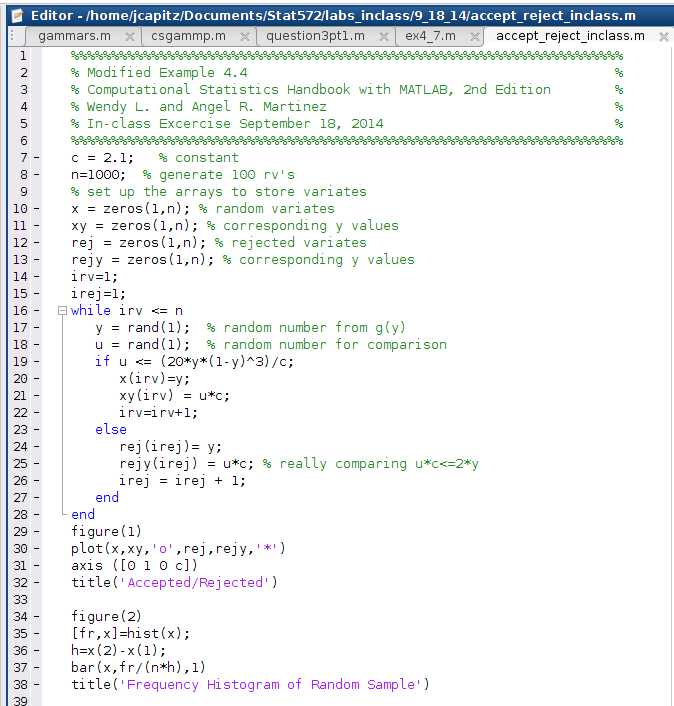
\includegraphics[scale=.50]{inClass2_acceptReject_code.png}
\caption{Code of the in-class Accept/Reject random sample exercise.}
\label{inclass2fig1}
\end{center}
\end{figure}
\FloatBarrier

\begin{figure}[ht!]
\begin{center}
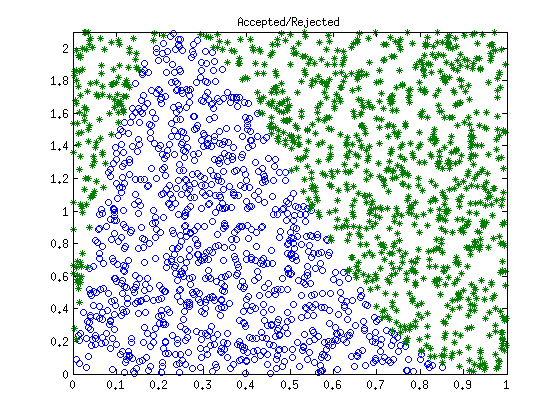
\includegraphics[scale=.80]{inClass2_acceptReject.png}
\caption{Plot of the in-class Accept/Reject random sample exercise.}
\label{inclass2fig2}
\end{center}
\end{figure}
\FloatBarrier

\begin{figure}[ht!]
\begin{center}
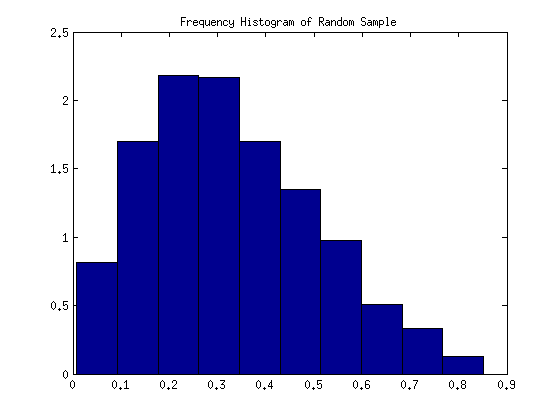
\includegraphics[scale=.80]{inClass2_acceptReject_hist.png}
\caption{Plot of the in-class Accept/Reject random sample exercise.}
\label{inclass2fig3}
\end{center}
\end{figure}
\FloatBarrier

\section*{Homework 3}

\subsection*{Exercise 4.6}

For this function I defined two input variables: $v$, which is the desired degrees of freedom for the chi-squared distribution and $n$, which is the desired sample size of the chi-square random variable. The simulation below is for $v=26$ and $n=1000$.
\begin{figure}[ht!]
\begin{center}
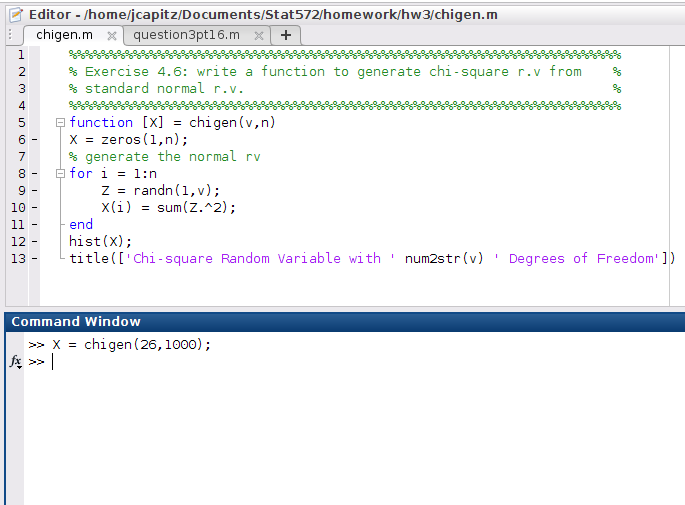
\includegraphics[scale=.70]{q4pt6_code.png}
\caption{Code for function chigen(). It generates Chi-square sample from standard normal sample.}
\label{q4pt6fig1}
\end{center}
\end{figure}
\FloatBarrier

\begin{figure}[ht!]
\begin{center}
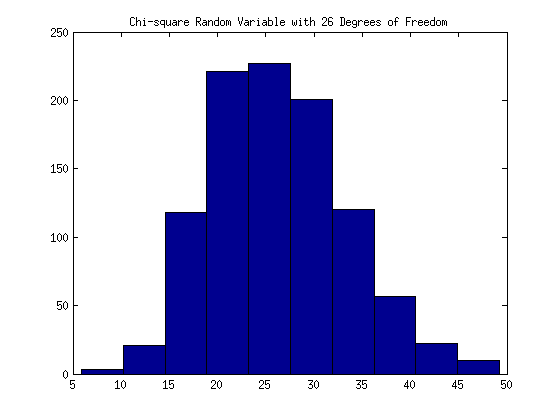
\includegraphics[scale=.80]{q4pt6_hist.png}
\caption{Chi-square random sample histogram, with $n=1000$ and 26 degrees of freedom.}
\label{q4pt6fig2}
\end{center}
\end{figure}
\FloatBarrier

\subsection*{Exercise 4.7}

This is an implementation of the algorithm described in exercise 4.7. Figure \ref{q4pt7fig1} shows the function I developed to implement the algorithm and generate random samples from the Beta distribution. The user needs to specify the sample size $n$, the parameters $\alpha$ and $\beta$. As an example I ran the algorithm with $n=10,000$ and $\alpha=3$, $\beta=3$, see figure \ref{q4pt7fig2}. I also ran it with $\alpha=0.333$, $\beta=0.333$, see figure \ref{q4pt7fig3}. Both histograms show that the random sample comes from a Beta distribution with the given parameters.

\begin{figure}[ht!]
\begin{center}
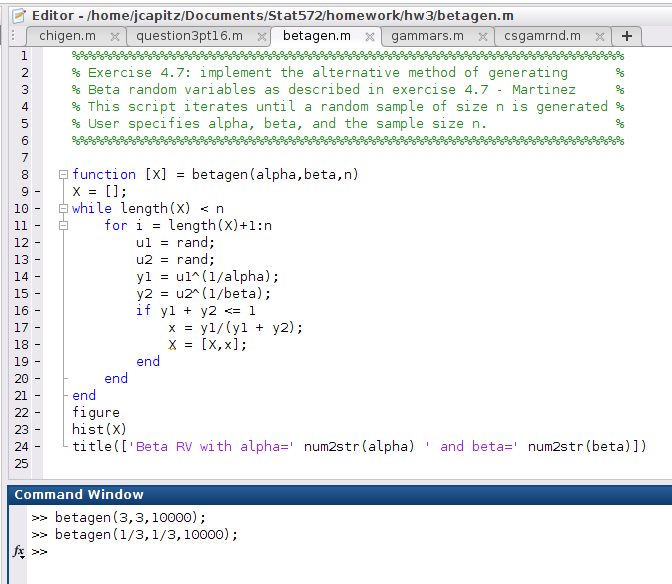
\includegraphics[scale=.60]{q4pt7_code.png}
\caption{}
\label{q4pt7fig1}
\end{center}
\end{figure}
\FloatBarrier

\begin{figure}[ht!]
\begin{center}
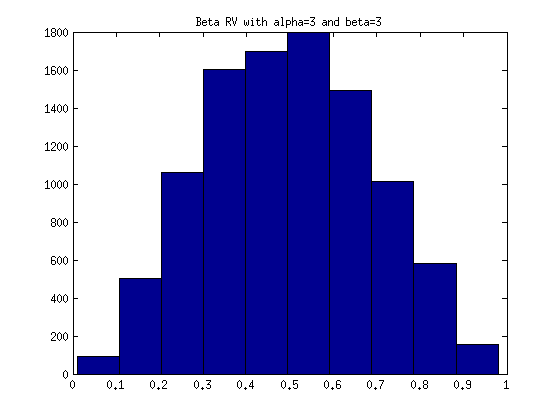
\includegraphics[scale=.80]{q4pt7_hist1.png}
\caption{Beta random sample, $\alpha=3$, $\beta=3$.}
\label{q4pt7fig2}
\end{center}
\end{figure}
\FloatBarrier

\begin{figure}[ht!]
\begin{center}
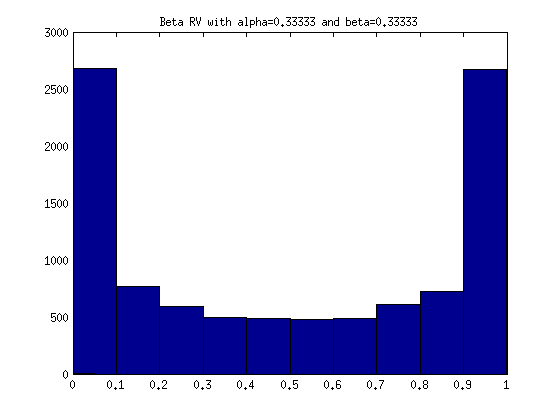
\includegraphics[scale=.80]{q4pt7_hist2.png}
\caption{Beta random sample, $\alpha=0.333$, $\beta=0.333$.}
\label{q4pt7fig3}
\end{center}
\end{figure}
\FloatBarrier

\subsection*{Exercise 4.8}

Rejected is the number of elements in the MATLAB vector $rej$. The number is $1,037$. As a percentage, the number of rejected is $\dfrac{1,037}{2,037}=0.5091$, or $50.91\%$. The probability that any value is accepted is given by $\displaystyle\sum_j P(j \text{ is accepted and } y = j)=\displaystyle\sum_j\dfrac{p_j}{c}=\dfrac{1}{c}$. Therefore, on average we need to generate $c$ values for $y$ before one is accepted. In this example $c=2$ and we observe an acceptance rate of about $50\%$, which is what would expect based on the theoretical probability of $\dfrac{1}{c}$. Figures \ref{q4pt8fig1} and \ref{q4pt8fig2} show code implementation and graphical results.

\begin{figure}[ht!]
\begin{center}
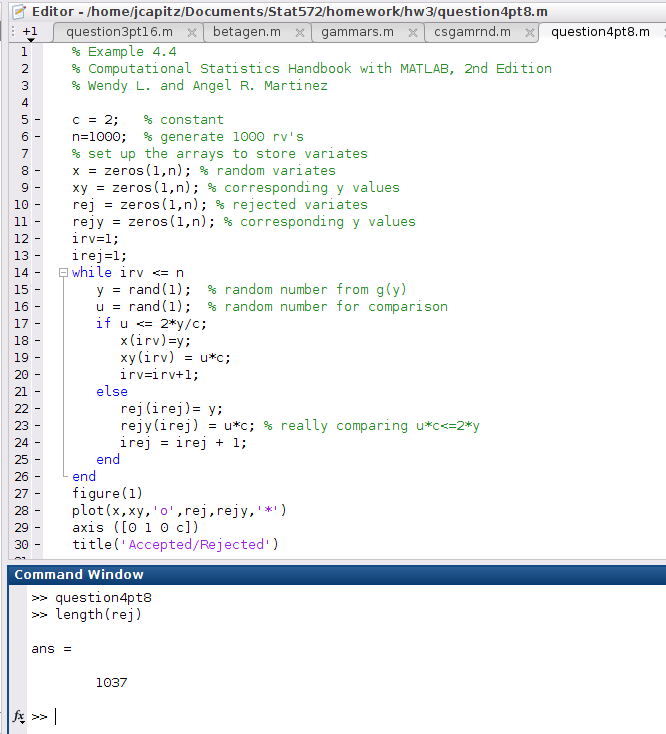
\includegraphics[scale=.60]{q4pt8_code.png}
\caption{}
\label{q4pt8fig1}
\end{center}
\end{figure}
\FloatBarrier

\begin{figure}[ht!]
\begin{center}
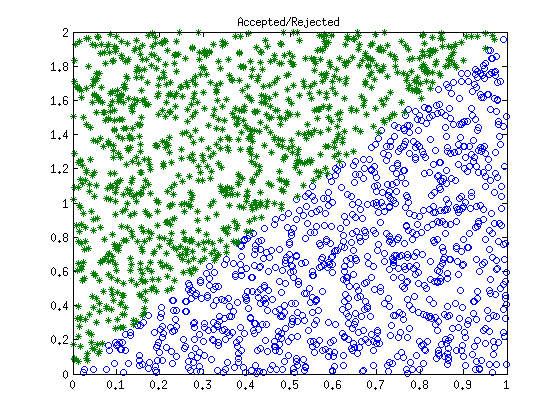
\includegraphics[scale=.80]{q4pt8_plot.png}
\caption{}
\label{q4pt8fig2}
\end{center}
\end{figure}
\FloatBarrier

\subsection*{Exercise 4.9}

In this exercise we generate a random sample of size $n=100$ from the probability mass function:
\[p(y)=\begin{cases}
0.15, & \text{if } Y=1\\
0.22 & \text{if } Y=2\\
0.33 & \text{if } Y=3\\
0.10 & \text{if } Y=4\\
0.20 & \text{if } Y=5\\
\end{cases}\]
Figure \ref{q4pt9fig1} shows the empirical results $f$ and the theoretical values $p$. We see that the distribution of the random closely matches said pmf. I also calculated the number of rejected vs accepted. Generated 191 variables and rejected 91, for a rejection ratio of $47.64\%$, which makes sense because $c=1.65$, so we expect to reject less than half. Figures \ref{q4pt9fig2} and \ref{q4pt9fig3} show the graphical results.


\begin{figure}[ht!]
\begin{center}
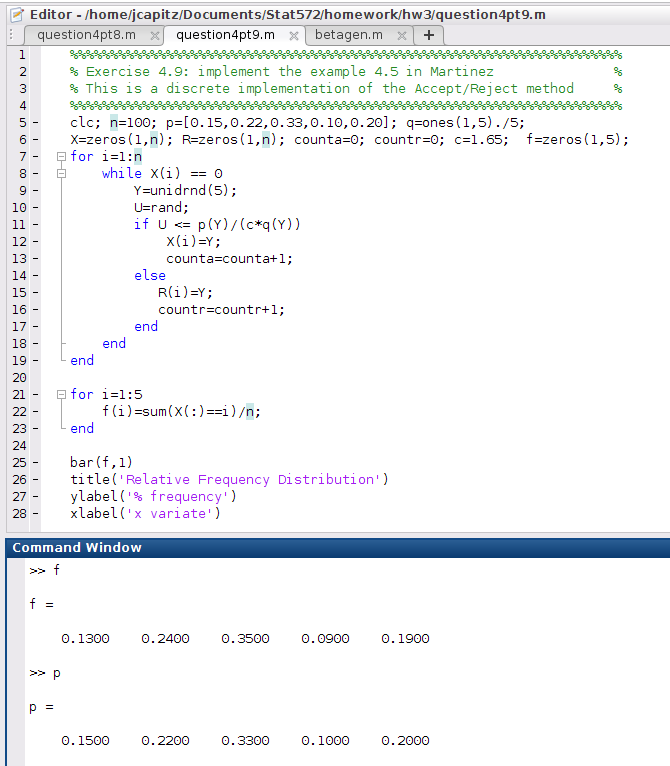
\includegraphics[scale=.60]{q4pt9_code.png}
\caption{}
\label{q4pt9fig1}
\end{center}
\end{figure}
\FloatBarrier

\begin{figure}[ht!]
\begin{center}
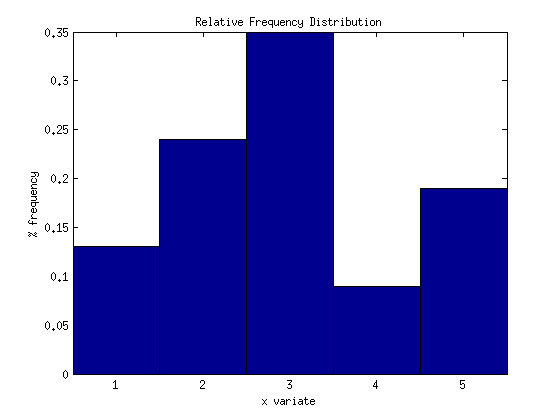
\includegraphics[scale=.80]{q4pt9_hist.png}
\caption{Empirical results of generating a discrete random sample from $p(y)$.}
\label{q4pt9fig2}
\end{center}
\end{figure}
\FloatBarrier

\begin{figure}[ht!]
\begin{center}
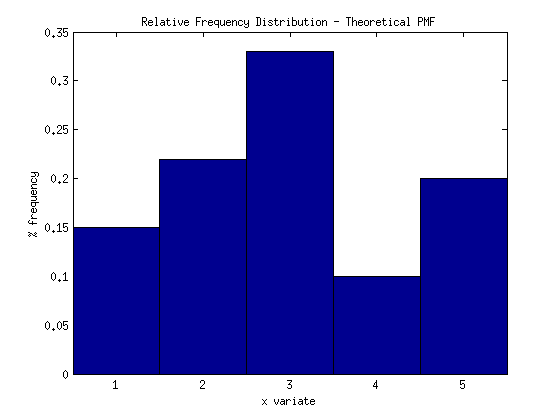
\includegraphics[scale=.80]{q4pt9_TheoreticalHist.png}
\caption{Theoretical frequency of $p(y)$}
\label{q4pt9fig3}
\end{center}
\end{figure}
\FloatBarrier

\end{document}